\documentclass[journal]{IEEEtran}
\usepackage{cite}
\usepackage{amsmath,amssymb}
\usepackage{graphicx}
\usepackage{booktabs}
\usepackage{array}
\usepackage{url}
\usepackage[hidelinks]{hyperref}
\hyphenation{state-of-health}

\begin{document}

\title{Cross-Dataset Generalization and Few-Shot Adaptation of Machine-Learning Models for Electric Vehicle Battery State-of-Health Estimation}

\author{Om~Manish~Makadia,
        Divyam~Jain,
        Goutham~T.~G.,
        D.~Pranav~Sai,
        and~M.~Dakshayini%
\thanks{The authors are with the Department of Artificial Intelligence and Machine Learning, B.M.S. College of Engineering, Bull Temple Road, Basavanagudi, Bengaluru 560019, Karnataka, India.}%
\thanks{Corresponding author: O. M. Makadia (e-mail: ommanish.ai23@bmsce.ac.in). Other e-mails: divyamjain.ai23@bmsce.ac.in, gouthamtaranagar.ai23@bmsce.ac.in, pranavsai.ai23@bmsce.ac.in, dakshayini.ise@bmsce.ac.in.}}

\markboth{Cross-dataset battery SOH estimation}{}
\maketitle

\begin{abstract}
State-of-health (SOH) estimators for lithium-ion batteries are usually validated inside a single laboratory dataset, so their transferability to other chemistries, cycling protocols and test regimes is poorly characterised. We present a battery-disjoint benchmark of cross-dataset SOH estimation on five public repositories (NASA, CALCE, XJTU, Oxford and MATR; 190 cells, 132,389 capacity observations) using the only predictor our harmonisation could guarantee in all five datasets, the cycle index. A training-mean baseline, Ridge, ElasticNet and XGBoost are evaluated in within-dataset, pairwise 5$\times$5 transfer, leave-one-dataset-out (LODO) and few-shot protocols over five seeds (6,120 executed runs plus 320 logged infeasible settings). Within a dataset, XGBoost reaches $3.89\pm3.19$ percentage points (pp) mean absolute error (MAE). Zero-shot transfer raises it to $13.03\pm8.45$ pp, which does not beat the training-mean baseline ($11.22\pm4.24$ pp); the baseline is at least as good in 12 of 20 source--target pairs. Linear models diverge when the target cycle range exceeds the source range, with errors up to 637 pp. Pooling four sources (LODO) bounds the error (10.82 pp) but still does not outperform the mean baseline (10.25 pp). Target labels help only from three support cells onward (on the three targets feasible at every $k$, XGBoost reaches 6.2 pp at $k{=}3$ and 5.0 pp at $k{=}10$, versus about 8 pp for a target-mean predictor), whereas label-free CORAL and mean--variance alignment do not (10.8--12.9 pp). Cross-dataset SOH claims should therefore be reported against a mean-baseline reference. Code and results are public.
\end{abstract}

\begin{IEEEkeywords}
State of health, Lithium-ion battery, Domain shift, Transfer learning, Benchmark, Generalization
\end{IEEEkeywords}

\section{Introduction}
\IEEEPARstart{L}{ithium-ion} batteries are the dominant energy-storage technology in electric vehicles (EVs) and stationary storage because of their high specific energy and falling cost. Their capacity fades with use, and the ratio of present to rated capacity, the state of health (SOH), determines usable range, safe charging limits and second-life value. Because capacity cannot be measured directly in operation, a battery management system (BMS) must estimate SOH from measurable signals~\cite{berecibar2016critical,hu2020battery,li2019datadriven}.

Data-driven estimators have become popular as public cycling datasets have grown. Machine-learning pipelines have reported low errors on cells from one laboratory, one chemistry and one test protocol~\cite{severson2019,roman2021,ng2020,zhang2020impedance}. A BMS in the field, however, meets cells that differ in chemistry, temperature, charging policy and usage. Transfer-learning studies address this shift~\cite{tan2020transfer,shen2020deep,ren2023novel,wang2024pinn}, and the BatteryLife benchmark evaluates models across aging conditions and domains for life prediction~\cite{tan2025batterylife}. What is still missing is a plain, leakage-controlled reference that shows how far the simplest estimators transfer across all pairs of widely used datasets, and whether they beat a trivial predictor when they do.

This paper supplies that reference. We harmonise five public repositories into one table and evaluate four regressors under four protocols, always splitting by whole cell so that no cell contributes to both training and testing~\cite{kaufman2012leakage,kapoor2023leakage}. Our contributions are as follows.
\begin{enumerate}
\item A reproducible benchmark on 190 cells and 132,389 observations, covering within-dataset, all 20 pairwise transfers, leave-one-dataset-out (LODO) and few-shot protocols, with a training-mean predictor as an explicit baseline in every protocol.
\item Evidence that within-dataset accuracy does not predict transferability: zero-shot XGBoost does not beat the mean baseline on average, and wins in only 8 of 20 pairs.
\item A diagnosis of linear-model failure as extrapolation beyond the source cycle range, supported by a rank correlation between range mismatch and error.
\item A comparison of label-based adaptation (training on $k$ target cells) with label-free alignment (CORAL and mean--variance normalisation), showing that only target labels help.
\item Open code, harmonised data and all result files, including the 320 settings that were infeasible because too few target cells exist.
\end{enumerate}
The data are laboratory cycling records, not fleet data; we do not claim field performance.

\section{Related Work}
\subsection{SOH estimation}
Model-based BMS methods track capacity through coulomb counting or equivalent-circuit models with Kalman filtering~\cite{plett2004ekf}. Data-driven methods learn the mapping from measured features to capacity, using Gaussian processes, support-vector machines, gradient-boosted trees and neural networks~\cite{li2019datadriven,hu2020battery}. High-profile studies predict cycle life from early-cycle voltage features~\cite{severson2019}, estimate health with a standardised machine-learning pipeline~\cite{roman2021}, or use impedance spectra~\cite{zhang2020impedance}. These works mostly report within-dataset errors.

\subsection{Transfer and domain adaptation}
Fine-tuning recurrent networks across cells~\cite{tan2020transfer}, ensembles of convolutional networks with transfer~\cite{shen2020deep}, universal health features with fine-tuning~\cite{ren2023novel} and physics-informed networks with transfer experiments~\cite{wang2024pinn} all report gains for a target domain. General surveys describe transfer learning~\cite{pan2010survey}, and correlation alignment (CORAL) matches second-order statistics of source and target inputs without target labels~\cite{sun2016coral}. Gulrajani and Lopez-Paz argued that domain-generalisation claims need careful baselines~\cite{gulrajani2021lost}, which motivates our use of a training-mean reference.

\subsection{Evaluation pitfalls}
Random splitting of cycles from the same cell leaks degradation trajectories between training and test sets~\cite{kaufman2012leakage,kapoor2023leakage}. We avoid this by splitting by cell and by excluding the current-cycle capacity and SOH from the inputs.

\section{Datasets and Label Harmonisation}
\subsection{Repositories}
Table~\ref{tab:data} summarises the five repositories. NASA contributes four 18650 cells~\cite{saha2007nasa}; CALCE contributes 15 prismatic CS2 cells~\cite{he2011calce}; XJTU contributes 23 NCM 18650 cells from the 2C and 3C batches of the 55-cell release~\cite{wang2024pinn}; Oxford contributes eight Kokam pouch cells aged at 40\,$^\circ$C under a dynamic driving profile, characterised every 100 cycles~\cite{birkl2017oxford}; and MATR contributes the LFP/graphite fast-charging dataset~\cite{severson2019}. The datasets differ by up to a factor of 49 in cycle span (168 cycles for NASA versus 8,200 for Oxford) and by chemistry, form factor, rated capacity, temperature and test protocol (Fig.~\ref{fig:data}).

\begin{table*}[!t]
\caption{Harmonised benchmark datasets. Obs. = capacity observations; EOL cells = cells with at least one observation below 80\% SOH (includes noisy CALCE records); RT = room temperature.}
\label{tab:data}
\centering
\scriptsize
\setlength{\tabcolsep}{4pt}
\begin{tabular}{llcccrrrcc}
\toprule
Dataset & Chemistry & Format & $Q_\mathrm{rated}$ (Ah) & Temp.\ ($^\circ$C) & Cells & Obs. & Max cycle & EOL cells & SOH (\%), mean\,$\pm$\,SD \\
\midrule
NASA & LCO/graphite & 18650 & 2.0 & 24 & 4 & 636 & 168 & 4 & 79.1\,$\pm$\,9.9 \\
CALCE & LCO/graphite & Prismatic & 1.1 & RT & 15 & 9,608 & 1,308 & 15 & 79.2\,$\pm$\,22.8 \\
XJTU & NCM/graphite & 18650 & 2.0 & RT & 23 & 6,938 & 419 & 4 & 93.4\,$\pm$\,4.8 \\
Oxford & LCO/graphite & Pouch & 0.74 & 40 & 8 & 519 & 8,200 & 8 & 86.1\,$\pm$\,6.7 \\
MATR & LFP/graphite & 18650 & 1.1 & 30 & 140 & 114,688 & 2,237 & 43 & 93.8\,$\pm$\,4.6 \\
\midrule
Total & & & & & 190 & 132,389 & & 74 & \\
\bottomrule
\end{tabular}
\end{table*}


\begin{figure*}[!t]
\centering
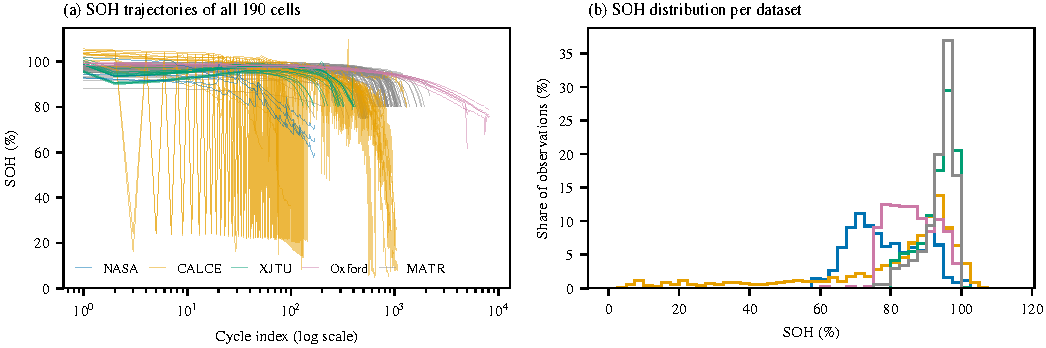
\includegraphics[width=\textwidth]{figs/Figure_1.pdf}
\caption{Heterogeneity of the five datasets. (a) SOH against cycle index (log scale) for all 190 cells; the Oxford series reaches 8,200 cycles whereas NASA ends at 168. Isolated low-SOH records in CALCE are discussed in Section~III-D. (b) Distribution of SOH observations per dataset.}
\label{fig:data}
\end{figure*}

\subsection{SOH label}
For each capacity-check event, SOH is the measured full-discharge capacity divided by the rated capacity,
\begin{equation}
\mathrm{SOH}_t=\frac{Q_t}{Q_\mathrm{rated}}\times 100\;[\%],
\label{eq:soh}
\end{equation}
with $Q_\mathrm{rated}$ taken from the source documentation (2.0\,Ah for NASA and XJTU, 1.1\,Ah for CALCE and MATR, 0.74\,Ah for Oxford). Values above 100\% are kept and labels are never interpolated; in particular, the Oxford series contains only the characterisation checkpoints (519 observations over 8 cells). Source-specific end-of-life definitions are preserved in the table, and observations below the end-of-life threshold are retained. For CALCE cells recorded with the CADEX tester, the capacity field is a progress percentage, so capacity is obtained by integrating discharge current over time.

\subsection{Input feature and leakage policy}
The harmonised table must contain only inputs that exist in every dataset. Charge-rate, voltage and current summaries are missing for at least one repository in our parsed table, and temperature is absent for XJTU. The only predictor available for all 190 cells is therefore the cycle index $c_t$, so each model estimates $\mathrm{SOH}_t=f(c_t)$. The measured capacity and SOH of the cycle being predicted never enter the input. This restriction makes the study a statement about cycle-index estimators, not about estimators that use voltage or current features; Section~\ref{sec:limits} discusses what this means.

\subsection{Data-quality notes}
Three properties of the data affect interpretation. (i) MATR supplies 87\% of all observations (114,688 of 132,389 rows) and has a narrow SOH range (mean 93.8\%, SD 4.6\%), and only 43 of its 140 cells fall below 80\% SOH; likewise only 4 of 23 XJTU cells do. (ii) CALCE labels are noisy: 1,201 of 9,608 observations (12.5\%) are below 50\% SOH, which probably reflects incomplete discharge segments in mixed-rate protocols. We therefore also report results without CALCE. (iii) Our parser returns 140 cell records for the three MATR batch files, whereas the original study analyses 124 cells~\cite{severson2019}; we keep all 140 records and have not tested sensitivity to this choice.

\section{Experimental Design}
\subsection{Models}
All models take the single input $c_t$ and are fixed in advance, without tuning. The \emph{Mean} baseline predicts the average training label. \emph{Ridge}~\cite{hoerl1970ridge} uses standardised inputs and $\ell_2$ penalty $\alpha=1$. \emph{ElasticNet}~\cite{zou2005elasticnet} uses $\alpha=0.01$ and $\ell_1$ ratio 0.5. \emph{XGBoost}~\cite{chen2016xgboost} uses 150 trees of depth 4, learning rate 0.05, row subsampling 0.8 and column subsampling 0.9. Sequence models are implemented in the repository but are not part of the results reported here.

\subsection{Protocols}
Fig.~\ref{fig:protocol} summarises the design. Every split is by whole cell. Training cells come from the source dataset(s) only, and the metric is the mean absolute error in SOH percentage points over all test observations,
\begin{equation}
\mathrm{MAE}=\frac{1}{N}\sum_{i=1}^{N}\left|y_i-\hat y_i\right|.
\label{eq:mae}
\end{equation}
Results are averaged over five seeds (11, 22, 33, 44, 55); a seed changes the cell split and the stochastic parts of XGBoost.


\begin{figure*}[!t]
\centering
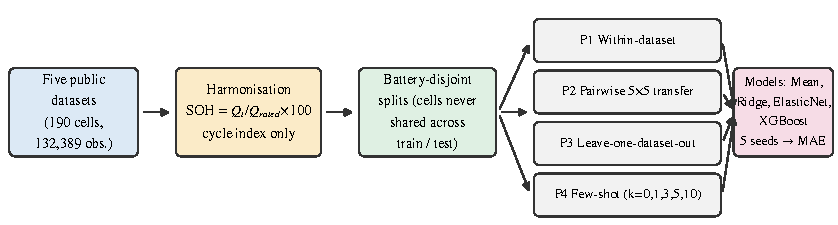
\includegraphics[width=\textwidth]{figs/Figure_2.pdf}
\caption{Experimental design. Five datasets are harmonised to a common SOH label and cycle-index input, split by whole cells, and evaluated under four protocols with four models over five seeds.}
\label{fig:protocol}
\end{figure*}

\emph{P1 Within-dataset.} Cells are split 25\% test, then 20\% of the remainder validation and the rest training (for example 9/2/4 cells for CALCE and 84/21/35 for MATR).

\emph{P2 Pairwise transfer.} A model trained on the training cells of source $S$ is evaluated, without any target data, on all cells of target $T\neq S$ (20 ordered pairs).

\emph{P3 LODO.} Training cells are the training splits of the four non-target datasets pooled; the fifth dataset is the target (30--112 training cells).

\emph{P4 Few-shot.} 30\% of target cells (at least two) are held out as the test set. From the rest, $k\in\{1,3,5,10\}$ support cells are drawn; $k=0$ is the unadapted source model. If fewer than $k$ support cells exist, the setting is logged as infeasible and not run. Four strategies are compared: \emph{scratch} (train on support cells only), \emph{pooled} (source training cells plus support cells), and two label-free alignments of the source input to the support input before training on source labels, \emph{mean--variance normalisation} and \emph{CORAL}~\cite{sun2016coral},
\begin{equation}
\tilde{X}_s=(X_s-\mu_s)\,A+\mu_t,\qquad A=(C_s+\lambda I)^{-1/2}(C_t+\lambda I)^{1/2},
\label{eq:coral}
\end{equation}
with $\lambda=10^{-3}$. With a single input feature, both alignments reduce to an affine rescaling of the cycle axis that uses no target labels.

The target-mean predictor, which predicts the mean label of the $k$ support cells, serves as the reference in P4. Counting only runs that actually executed, the study contains 500 matrix runs, 100 LODO runs and 5,520 few-shot runs (6,120 in total); a further 320 few-shot settings (NASA with $k\ge3$ and Oxford with $k=10$) are logged as infeasible.

\section{Results}
\subsection{Within-dataset accuracy}
Table~\ref{tab:within} shows that XGBoost attains the lowest within-dataset error ($3.89\pm3.19$ pp over 25 runs), ahead of Ridge ($4.51\pm3.72$) and ElasticNet ($4.52\pm3.72$), while the training mean gives $7.87\pm5.06$. Relative to the mean baseline, XGBoost reduces error by 79\% on Oxford, 54\% on XJTU, 53\% on NASA, 44\% on CALCE and only 24\% on MATR. Low absolute errors on MATR and XJTU therefore partly reflect their narrow SOH range (SD below 5 pp), not only model skill. CALCE is hardest (9.40 pp for XGBoost), consistent with its noisy labels.

\begin{table}[!t]
\caption{Within-dataset test MAE (pp), mean\,$\pm$\,SD over 5 seeds. Best per row in bold.}
\label{tab:within}
\centering
\scriptsize
\setlength{\tabcolsep}{3pt}
\begin{tabular}{lcccc}
\toprule
Dataset & Mean & Ridge & ElasticNet & XGBoost \\
\midrule
NASA & 9.09\,$\pm$\,2.09 & 4.41\,$\pm$\,1.60 & 4.41\,$\pm$\,1.59 & \textbf{4.29\,$\pm$\,1.39} \\
CALCE & 16.71\,$\pm$\,1.67 & 11.25\,$\pm$\,2.06 & 11.27\,$\pm$\,2.05 & \textbf{9.40\,$\pm$\,2.20} \\
XJTU & 3.93\,$\pm$\,0.07 & 2.39\,$\pm$\,0.20 & 2.39\,$\pm$\,0.20 & \textbf{1.82\,$\pm$\,0.25} \\
Oxford & 6.04\,$\pm$\,0.29 & 1.72\,$\pm$\,0.50 & 1.73\,$\pm$\,0.50 & \textbf{1.25\,$\pm$\,0.35} \\
MATR & 3.58\,$\pm$\,0.17 & 2.77\,$\pm$\,0.20 & 2.78\,$\pm$\,0.20 & \textbf{2.71\,$\pm$\,0.22} \\
\midrule
All (25 runs) & 7.87\,$\pm$\,5.06 & 4.51\,$\pm$\,3.72 & 4.52\,$\pm$\,3.72 & \textbf{3.89\,$\pm$\,3.19} \\
\bottomrule
\end{tabular}
\end{table}

\subsection{Pairwise zero-shot transfer}
Table~\ref{tab:cross} and Fig.~\ref{fig:matrix} give the 20 transfers. Averaged over pairs and seeds, zero-shot MAE is $13.03\pm8.45$ pp for XGBoost, $61.49\pm138.98$ for Ridge, $61.31\pm138.63$ for ElasticNet and $11.22\pm4.24$ for the training mean. The mean baseline is better than XGBoost on average and in 12 of 20 pairs; XGBoost beats it in 8 pairs and Ridge in 6. Transfer works in a few pairs: MATR$\to$XJTU (Ridge 3.43 pp versus mean 3.80), CALCE$\to$XJTU (Ridge 3.87 versus 13.89), and Oxford$\to$MATR, where Ridge and XGBoost reach 2.73 and 2.87 pp against 8.10 for the mean and 2.71 for XGBoost trained within MATR. We regard this Oxford$\to$MATR result as a coincidence of fade shape over the first 2,000 cycles; our data cannot support an electrochemical explanation, because chemistry, temperature, protocol and cycle span all differ.

\begin{table*}[!t]
\caption{Zero-shot pairwise transfer, test MAE (pp), mean\,$\pm$\,SD over 5 seeds. The model is trained on the source and evaluated on all target cells. Best of the three per pair in bold; ElasticNet is within 1.6 pp of Ridge in every pair and is in the released result files.}
\label{tab:cross}
\centering
\scriptsize
\setlength{\tabcolsep}{3.5pt}
\begin{tabular}{lccc@{\hspace{14pt}}lccc}
\toprule
Source$\to$Target & Mean & Ridge & XGBoost & Source$\to$Target & Mean & Ridge & XGBoost \\
\midrule
NASA$\to$CALCE & \textbf{17.0\,$\pm$\,0.3} & 68.5\,$\pm$\,8.0 & 20.4\,$\pm$\,1.2 & XJTU$\to$Oxford & 8.2\,$\pm$\,0.1 & 110\,$\pm$\,5 & \textbf{5.8\,$\pm$\,0.0} \\
NASA$\to$XJTU & \textbf{13.5\,$\pm$\,0.9} & 28.6\,$\pm$\,2.1 & 18.9\,$\pm$\,1.7 & XJTU$\to$MATR & \textbf{3.6\,$\pm$\,0.1} & 11.7\,$\pm$\,0.4 & 7.7\,$\pm$\,0.0 \\
NASA$\to$Oxford & \textbf{7.4\,$\pm$\,0.5} & 637\,$\pm$\,76 & 17.1\,$\pm$\,2.7 & Oxford$\to$NASA & \textbf{10.4\,$\pm$\,0.1} & 17.0\,$\pm$\,0.2 & 19.6\,$\pm$\,0.2 \\
NASA$\to$MATR & \textbf{14.0\,$\pm$\,0.9} & 86.0\,$\pm$\,8.6 & 23.1\,$\pm$\,2.3 & Oxford$\to$CALCE & \textbf{15.4\,$\pm$\,0.0} & 16.7\,$\pm$\,0.1 & 17.6\,$\pm$\,0.1 \\
CALCE$\to$NASA & \textbf{8.7\,$\pm$\,0.2} & 15.1\,$\pm$\,1.9 & 10.7\,$\pm$\,1.4 & Oxford$\to$XJTU & 7.7\,$\pm$\,0.2 & \textbf{3.6\,$\pm$\,0.0} & 4.7\,$\pm$\,0.2 \\
CALCE$\to$XJTU & 13.9\,$\pm$\,2.3 & \textbf{3.9\,$\pm$\,0.9} & 5.6\,$\pm$\,1.0 & Oxford$\to$MATR & 8.1\,$\pm$\,0.2 & \textbf{2.7\,$\pm$\,0.0} & 2.9\,$\pm$\,0.1 \\
CALCE$\to$Oxford & \textbf{7.7\,$\pm$\,1.5} & 134\,$\pm$\,45 & 18.9\,$\pm$\,26.6 & MATR$\to$NASA & \textbf{15.0\,$\pm$\,0.0} & 17.5\,$\pm$\,0.0 & 18.2\,$\pm$\,0.1 \\
CALCE$\to$MATR & \textbf{14.4\,$\pm$\,2.3} & 16.2\,$\pm$\,3.6 & 14.7\,$\pm$\,4.1 & MATR$\to$CALCE & 16.4\,$\pm$\,0.0 & 15.7\,$\pm$\,0.1 & \textbf{15.5\,$\pm$\,0.1} \\
XJTU$\to$NASA & \textbf{14.6\,$\pm$\,0.1} & 17.1\,$\pm$\,0.3 & 17.1\,$\pm$\,0.3 & MATR$\to$XJTU & 3.8\,$\pm$\,0.0 & \textbf{3.4\,$\pm$\,0.0} & 3.6\,$\pm$\,0.0 \\
XJTU$\to$CALCE & 16.2\,$\pm$\,0.1 & \textbf{11.5\,$\pm$\,0.0} & 13.0\,$\pm$\,0.0 & MATR$\to$Oxford & 8.5\,$\pm$\,0.0 & 12.9\,$\pm$\,1.1 & \textbf{5.6\,$\pm$\,0.6} \\
\bottomrule
\end{tabular}
\end{table*}

\begin{figure*}[!t]
\centering
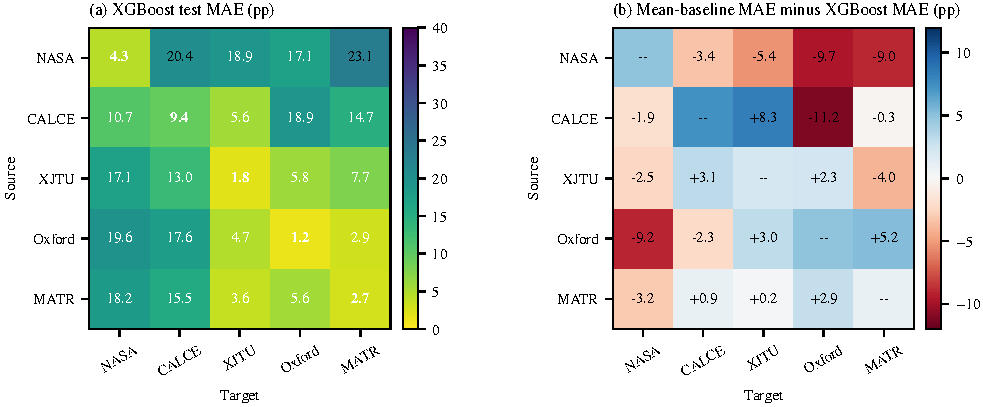
\includegraphics[width=\textwidth]{figs/Figure_3.pdf}
\caption{Cross-dataset transfer with XGBoost. (a) Test MAE; diagonal entries are within-dataset holdout results and colour is capped at 40 pp. (b) Mean-baseline MAE minus XGBoost MAE; blue means XGBoost is better than predicting the training mean, red means worse.}
\label{fig:matrix}
\end{figure*}

\subsection{Linear extrapolation failure}
Ridge and ElasticNet errors exceed 100 pp in three pairs (NASA$\to$Oxford $637.45\pm75.52$, CALCE$\to$Oxford 133.77, XJTU$\to$Oxford 110.49), all with Oxford as the target. A linear fit on the four NASA cells has slope $-0.196$\,\%/cycle and predicts $-1{,}511\%$ at cycle 8,200, the end of the Oxford series (Fig.~\ref{fig:extrap}a). A tree ensemble returns the value of its last leaf outside the training range (about 66\% here), so XGBoost stays bounded, at $17.10\pm2.67$ pp for NASA$\to$Oxford. The ratio of target to source maximum cycle index explains part of this: across the 20 pairs the Spearman correlation with Ridge error is $\rho=0.55$ ($p=0.012$), against $0.23$ ($p=0.33$) for XGBoost and $-0.07$ for the mean (Fig.~\ref{fig:extrap}b). The pairs are not independent, so $p$ is descriptive only.

\begin{figure*}[!t]
\centering
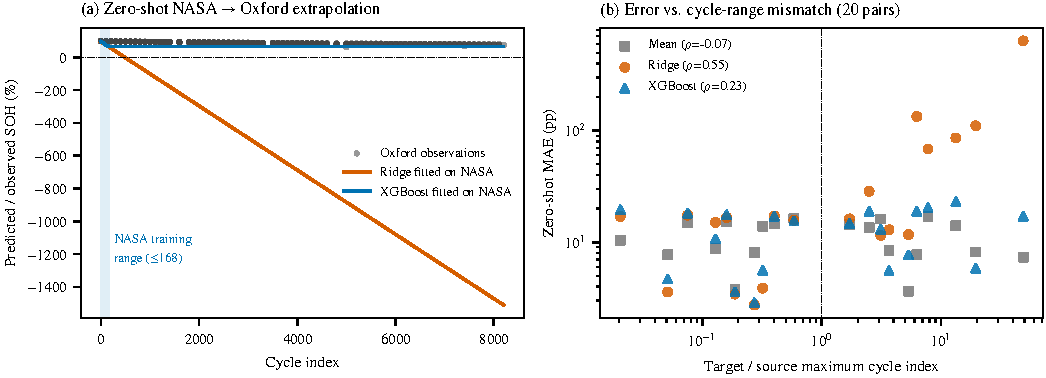
\includegraphics[width=\textwidth]{figs/Figure_4.pdf}
\caption{Why linear models fail across datasets. (a) Models fitted on the four NASA cells and extrapolated to the Oxford cycle range (illustration with all NASA cells; the experiments use seeded training splits). (b) Zero-shot MAE against the ratio of target to source maximum cycle index for all 20 pairs.}
\label{fig:extrap}
\end{figure*}

\subsection{Leave-one-dataset-out}
Table~\ref{tab:lodo} shows that pooling bounds the error: the largest LODO error is 19.1 pp, against 637 pp for single-source linear transfer. Averaged over 25 runs, however, the mean baseline ($10.25\pm4.47$ pp) remains slightly better than XGBoost ($10.82\pm5.44$), Ridge ($12.72\pm5.84$) and ElasticNet ($12.69\pm5.80$). Models beat the mean on XJTU, Oxford (XGBoost 5.88 versus 7.69; Ridge fails with 19.08) and CALCE, while the mean wins on MATR and NASA. Because MATR contributes 84 of the 105 training cells when CALCE is held out, and 87\% of all rows, pooled training is dominated by MATR; LODO should be read as ``trained mostly on MATR'' for non-MATR targets.

\begin{table*}[!t]
\caption{Leave-one-dataset-out test MAE (pp), mean\,$\pm$\,SD over 5 seeds. Train cells = pooled cells of the four source datasets. Best per row in bold.}
\label{tab:lodo}
\centering
\scriptsize
\setlength{\tabcolsep}{5pt}
\begin{tabular}{lccccc}
\toprule
Held-out target & Train cells & Mean & Ridge & ElasticNet & XGBoost \\
\midrule
NASA & 112 & \textbf{13.95\,$\pm$\,0.04} & 16.16\,$\pm$\,0.36 & 16.14\,$\pm$\,0.36 & 17.34\,$\pm$\,0.20 \\
CALCE & 105 & 16.29\,$\pm$\,0.05 & 15.69\,$\pm$\,0.11 & 15.69\,$\pm$\,0.11 & \textbf{15.38\,$\pm$\,0.15} \\
XJTU & 100 & 4.17\,$\pm$\,0.07 & \textbf{3.29\,$\pm$\,0.06} & 3.30\,$\pm$\,0.06 & 3.60\,$\pm$\,0.08 \\
Oxford & 109 & 7.69\,$\pm$\,0.03 & 19.08\,$\pm$\,1.34 & 18.91\,$\pm$\,1.34 & \textbf{5.88\,$\pm$\,0.67} \\
MATR & 30 & \textbf{9.13\,$\pm$\,1.12} & 9.40\,$\pm$\,1.25 & 9.39\,$\pm$\,1.25 & 11.92\,$\pm$\,0.75 \\
\midrule
All (25 runs) & & \textbf{10.25\,$\pm$\,4.47} & 12.72\,$\pm$\,5.84 & 12.69\,$\pm$\,5.80 & 10.82\,$\pm$\,5.44 \\
\bottomrule
\end{tabular}
\end{table*}

\subsection{Few-shot adaptation}
Table~\ref{tab:fewshot} averages over the three targets that remain feasible for every $k$ (CALCE, MATR, XJTU), so that columns are comparable; per-target curves are in Fig.~\ref{fig:fewshot}. With one support cell, no method beats predicting that cell's mean label (8.53 pp); XGBoost trained from scratch gives 10.78 pp and Ridge 21.46 pp. From $k=3$, training on target labels clearly helps: XGBoost from scratch reaches 6.22, 5.12 and 4.98 pp at $k=3,5,10$ against about 8 pp for the target mean, and a pooled model is 1.0--1.4 pp worse than scratch for $k\ge3$. The label-free alignments do not help at any $k$ (10.8--12.9 pp) and are no better than the unadapted model ($12.11$ pp), which is expected: with one feature they only rescale the cycle axis and never see a target SOH label. CORAL and normalisation differ by 0.01 pp on average (largest difference 0.71 pp). Including every target where a setting was feasible, XGBoost from scratch gives 7.75 pp at $k{=}1$ and 4.16 pp at $k{=}5$, against 13.08 pp zero-shot, but this average mixes different target sets across $k$ (Section~\ref{sec:design-note}).

\begin{table}[!t]
\caption{Few-shot test MAE (pp) averaged over CALCE, MATR and XJTU targets, all four sources and 5 seeds. $k=0$ is the unadapted source model (target mean: training mean).}
\label{tab:fewshot}
\centering
\scriptsize
\setlength{\tabcolsep}{4pt}
\begin{tabular}{lccccc}
\toprule
Method & $k{=}0$ & $k{=}1$ & $k{=}3$ & $k{=}5$ & $k{=}10$ \\
\midrule
Mean (target mean) & 11.84 & 8.53 & 8.11 & 8.21 & 8.03 \\
Ridge, from scratch & 21.89 & 21.46 & 6.55 & 6.02 & 5.69 \\
Ridge, pooled & 21.89 & 12.29 & 8.02 & 7.48 & 6.98 \\
XGBoost, from scratch & 12.11 & 10.78 & 6.22 & 5.12 & 4.98 \\
XGBoost, pooled & 12.11 & 10.00 & 7.52 & 6.54 & 5.96 \\
XGBoost, CORAL & 12.11 & 12.88 & 11.02 & 10.90 & 10.82 \\
XGBoost, mean--var. norm. & 12.11 & 12.88 & 11.02 & 10.90 & 10.82 \\
\bottomrule
\end{tabular}
\end{table}

\begin{figure*}[!t]
\centering
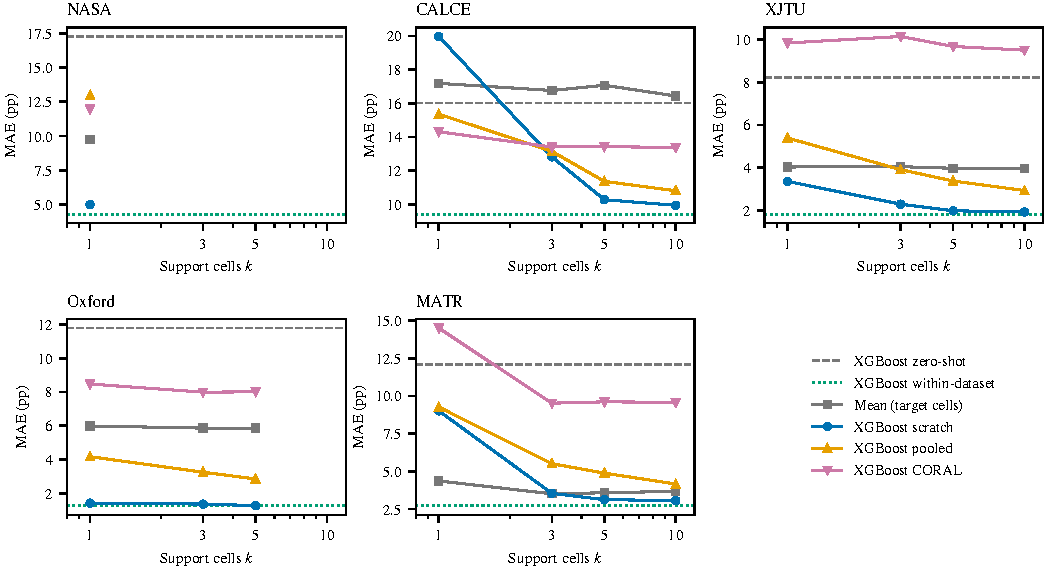
\includegraphics[width=0.92\textwidth]{figs/Figure_5.pdf}
\caption{Few-shot adaptation per target dataset (XGBoost), averaged over source datasets and seeds. NASA is feasible only for $k=1$ and Oxford up to $k=5$ because the target pool is small.}
\label{fig:fewshot}
\end{figure*}

\subsection{Robustness to CALCE}
Removing every pair that involves CALCE leaves 12 pairs. Mean absolute errors are then 9.57 pp for the mean baseline, 12.01 pp for XGBoost and 79.04 pp for Ridge, with XGBoost better than the mean in 5 of 12 pairs and Ridge in 3. The ordering is unchanged, so the main conclusions do not depend on the noisy CALCE labels.

\section{Discussion}
\subsection{What the results say}
A cycle-index model captures how fast cells of one dataset age, and that rate is a property of the dataset, not of battery health in general. When the target ages at a different rate or over a different span, the source model transfers a wrong calendar, and a constant is often a better guess. Within-dataset accuracy is thus a poor predictor of transferability, and it should be accompanied by a mean-baseline reference. Our LODO and few-shot results suggest two practical ideas for BMS design, with the caveat that they come from cycle-index models on laboratory cells: bounding the output range (SOH clipped to a physical interval) removes the divergence of linear models, and a handful of labelled target cells is far more useful than unlabeled alignment.

\subsection{Design note}
\label{sec:design-note}
The test set of the few-shot protocol is a 30\% subset of target cells, so the $k{=}0$ error (13.08 pp) differs slightly from the pairwise zero-shot error on all target cells (13.03 pp). The number of feasible targets also shrinks with $k$, which is why Table~\ref{tab:fewshot} fixes the target set. MAE is computed over observations, so datasets and cells with many cycles weigh more; a per-cell macro average was not computed.

\subsection{Limitations}
\label{sec:limits}
\begin{enumerate}
\item \emph{Single predictor.} Conclusions concern cycle-index estimators. Estimators using voltage, current or partial-charge features may transfer better; testing this requires re-extracting features from the raw files of all five datasets, which we have not done.
\item \emph{Small pools.} NASA has four cells and Oxford eight, so test sets and support pools are tiny (two and three test cells in P4), and seed variability is high for these targets.
\item \emph{Data quality.} CALCE labels are noisy (Section~III-D), and MATR cell counts differ from the original study. MATR dominates pooled training.
\item \emph{Confounding.} Chemistry, temperature, protocol and cycle span change together across datasets, so we report associations (for example the rank correlation in Fig.~\ref{fig:extrap}b), not causes.
\item \emph{Uncertainty and tuning.} Reported spreads are standard deviations across seeds, not confidence intervals; hyperparameters were fixed, and sequence models are not evaluated.
\item \emph{Laboratory data.} No fleet or vehicle data are used.
\end{enumerate}

\section{Conclusion}
On 190 cells from five public datasets, a cycle-index SOH estimator that is accurate within its own dataset (3.89 pp MAE for XGBoost) does not transfer: zero-shot XGBoost makes 13.03 pp error and does not beat the training mean (11.22 pp), unconstrained linear models diverge when the target cycle range exceeds the source's, and pooling four sources bounds the error without beating the mean. Labelled target cells help from $k=3$, whereas label-free alignment does not. We recommend reporting a training-mean baseline and the source-to-target cycle-range ratio in any cross-dataset SOH study, and treating richer feature sets, harmonised across repositories, as the next step. The code, harmonised table and all results are public, including the settings that were infeasible.

\section*{CRediT Author Statement}
\textbf{O. M. Makadia:} Conceptualization, Software, Formal analysis, Visualization, Writing -- original draft, Project administration. \textbf{D. Jain:} Data curation, Software, Investigation. \textbf{G. T. G.:} Investigation, Validation, Writing -- review \& editing. \textbf{D. P. Sai:} Data curation, Methodology, Writing -- review \& editing. \textbf{M. Dakshayini:} Supervision, Writing -- review \& editing.

\section*{Declaration of Generative AI and AI-Assisted Technologies in the Manuscript Preparation Process}
During the preparation of this work the authors used Google Antigravity to assist in writing the software code for the experiments, and Claude (Anthropic) to assist in drafting and editing the manuscript and in writing the scripts that generate its figures and tables. After using these tools, the authors reviewed and edited the content as needed and take full responsibility for the content of the published article.

\section*{Funding}
This research did not receive any specific grant from funding agencies in the public, commercial, or not-for-profit sectors.

\section*{Declaration of Competing Interest}
The authors declare that they have no known competing financial interests or personal relationships that could have appeared to influence the work reported in this paper.

\section*{Data and Code Availability}
The source datasets are public: NASA PCoE battery data~\cite{saha2007nasa} (\url{https://www.nasa.gov/content/prognostics-center-of-excellence-data-set-repository}); CALCE CS2 (\url{https://calce.umd.edu/battery-data}); XJTU (\url{https://zenodo.org/records/10963339}); Oxford Battery Degradation Dataset 1 (\url{https://ora.ox.ac.uk/objects/uuid:03ba4b01-cfed-46d3-9b1a-7d4a7bdf6fac}); and MATR (\url{https://data.matr.io/1/projects/5c48dd2bc625d700019f3204}). The raw files total about 11.7\,GB and are not redistributed. The code, the harmonised table (\texttt{data/processed/unified.csv}), and all result files and figure sources are available at \url{https://github.com/om-makadia-118/ev-battery-soh}.

\section*{Acknowledgements}
The authors thank the Department of Artificial Intelligence and Machine Learning, B.M.S. College of Engineering, for support during Project Work 2, and the groups that released the five datasets.

\bibliographystyle{IEEEtran}
\bibliography{refs}

\end{document}
